\documentclass{article}

\usepackage{KjelsethReportStyle}

%   ############################## Customisation ##############################

% Document metadata
\title{\fontsize{24}{36}\selectfont Programable Logic Circuts\\ %Edit title here \\ means new line
Lab 05} % Line 2 of title, its not subtitle, that is possible to, google it
\author{{\ttfamily Sølve Kjelseth}} % Input your name, replace \ttfamily with \normalfont to make it not monospaced but regular font (removing \ttfamily will not do this because of the monospaced font inside tables command, and author is technically a 1x1 table)
\date{\today} % Auto updates the date, untill you export it, replace with hardcoded date if you need

%   ############################## Document begins here ##############################
\begin{document}

\maketitle % Makes title front page based on the title, author and date metadata, change at the top



%   ############################## Section ##############################
\addtocontents{toc}{\protect\setcounter{tocdepth}{0}} % Temporarily hide from TOC
\section{Introduction} % Numbered section named Introduction
This is the fifth report in this course, detailing the completion of the fifth lab exercise. With the purpose is to investigate generics and counters.\par
Note: As always, the \LaTeX\ code is open source, see
\linkgithub{my GitHub {
\begingroup
\setbox0=\hbox{\includegraphics[scale=0.5]{Figures/github-mark.png}}%
\parbox{\wd0}{\box0}
\endgroup}}
\clearpage
\tableofcontents % Generate TOC
\clearpage
\listoffigures % List of figures
%\clearpage
%\listoftables % List of tables
\addtocontents{toc}{\protect\setcounter{tocdepth}{2}} % Restore TOC depth



%   ############################## Section ##############################
\section{Part 1}
This Part is about making a generic counter with a desired rollover value. Then instancing it to check the function.


\subsection{Solving}
Solving this task was done by first making a generic counter and then add a clause to reset the counter when the rollover value was reached and output a signal. Then the counter was instanced in the TLE with a generic map in addition to the port map to show the function.


\clearpage
\subsection{Code}
\writecode[VHDL]{Part1_TLE.vhd}{TLE for testing counter and rollover}

\clearpage
\writecode[VHDL]{Part1_mod_k.vhd}{Generic counter component used in the TLE}


\subsection{RTL}

\begin{figure}[h]
    \centering
    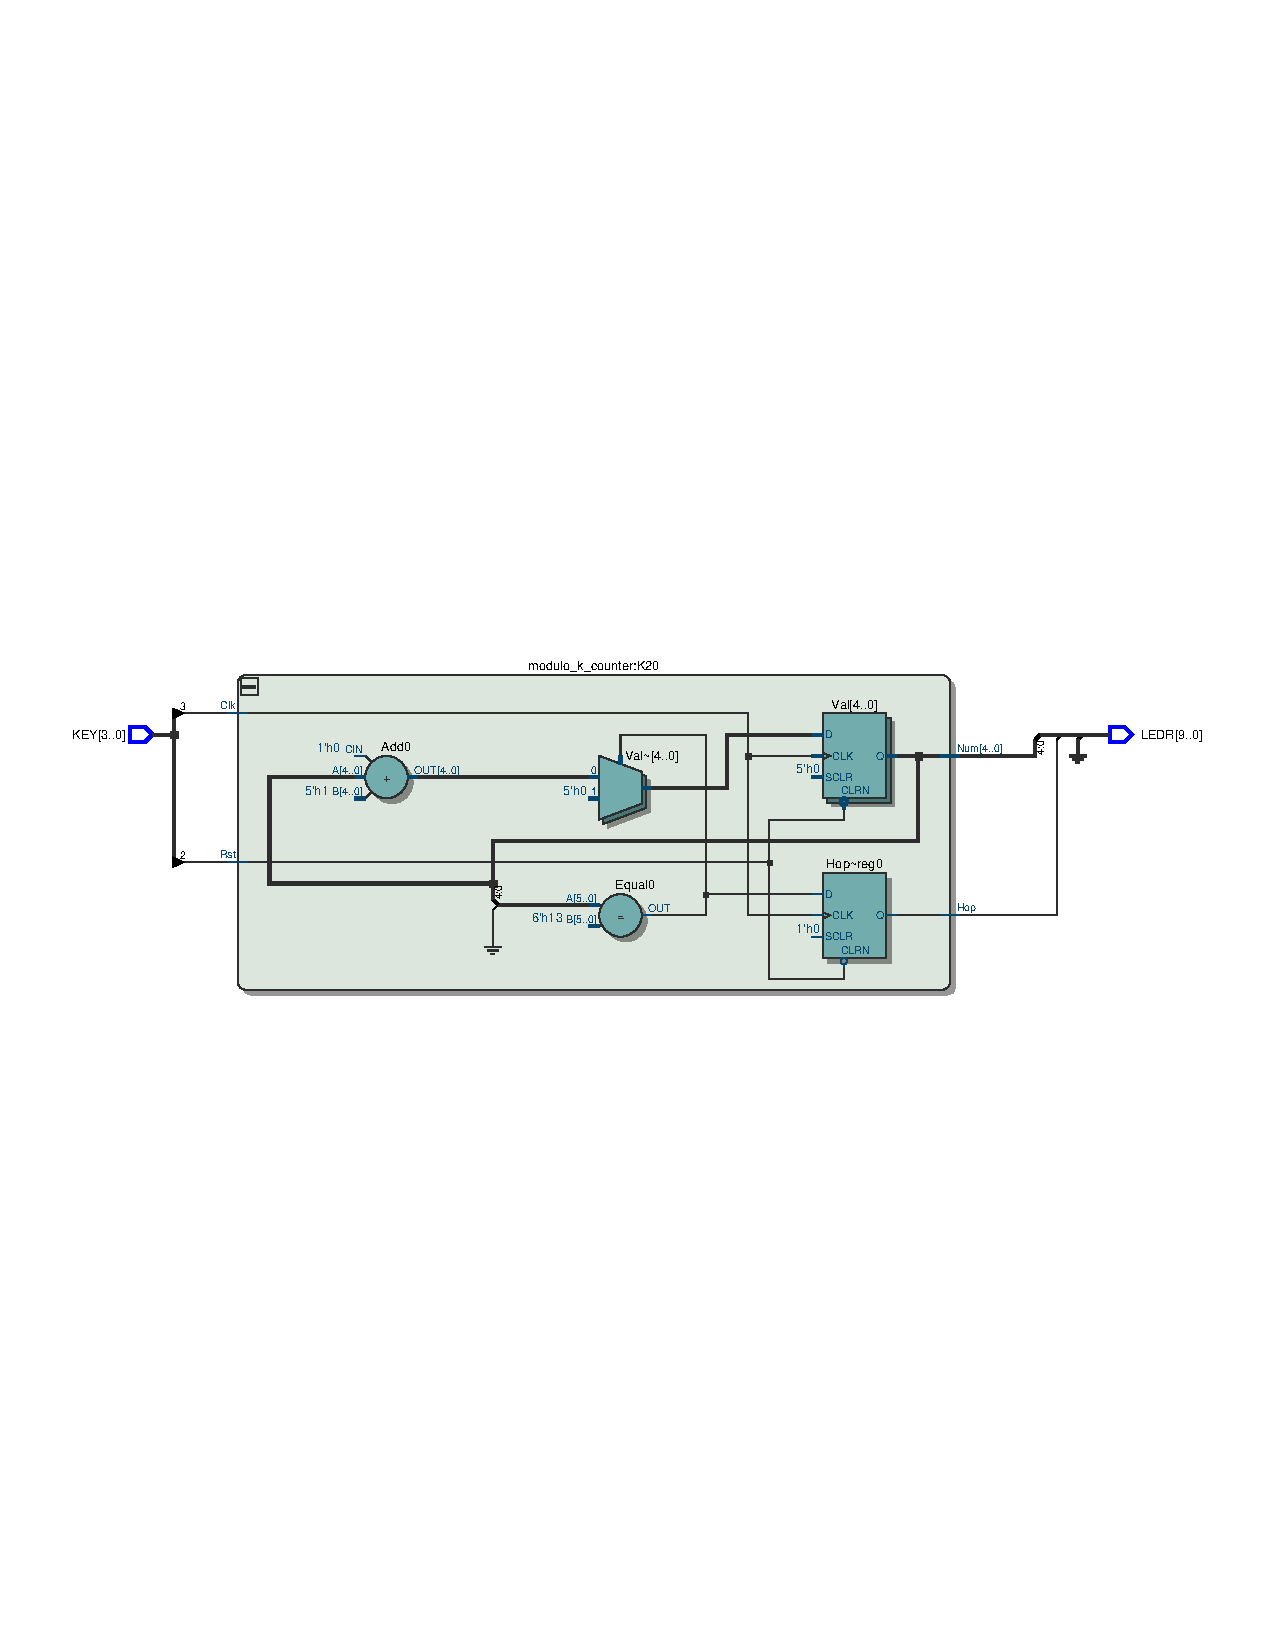
\includegraphics[width=1\textwidth]{Figures/Part1_RTL.jpg}
    \figcaption{RTL of the TLE with counter}
    \label{fig:p1_RTL_TLE}
\end{figure}

\clearpage
\subsection{Results}

\begin{figure}[ht]
    \centering
    \begin{subfigure}[t]{1\textwidth}
        \centering
        \includegraphics[width=0.8\textwidth]{Figures/Part1_1.jpg}
        \caption{Default state}
        \label{fig:p1_1}
    \end{subfigure}

    \begin{subfigure}[t]{1\textwidth}
        \centering
        \includegraphics[width=0.8\textwidth]{Figures/Part1_2.jpg}
        \caption{Clock cycle 1, counts up}
        \label{fig:p1_2}
    \end{subfigure}

    \begin{subfigure}[t]{1\textwidth}
        \centering
        \includegraphics[width=0.8\textwidth]{Figures/Part1_3.jpg}
        \caption{Clock cycle 2, counts up}
        \label{fig:p1_3}
    \end{subfigure}

    \begin{subfigure}[t]{1\textwidth}
        \centering
        \includegraphics[width=0.8\textwidth]{Figures/Part1_4.jpg}
        \caption{Clock cycle 3, counts up}
        \label{fig:p1_4}
    \end{subfigure}

    \figcaption{Function test, works as expected}
    \label{fig:p1_results}
\end{figure}

\clearpage
\begin{figure}[h]\ContinuedFloat
    \centering
    \begin{subfigure}[t]{1\textwidth}
        \centering
        \includegraphics[width=0.8\textwidth]{Figures/Part1_5.jpg}
        \caption{Clock cycle 19, counts up}
        \label{fig:p1_5}
    \end{subfigure}

    \begin{subfigure}[t]{1\textwidth}
        \centering
        \includegraphics[width=0.8\textwidth]{Figures/Part1_6.jpg}
        \caption{Clock cycle 20, resets to 0 and sets rollover flag}
        \label{fig:p1_6}
    \end{subfigure}

    \begin{subfigure}[t]{1\textwidth}
        \centering
        \includegraphics[width=0.8\textwidth]{Figures/Part1_7.jpg}
        \caption{Clock cycle 21, counts up and clears rollover flag}
        \label{fig:p1_7}
    \end{subfigure}

    \begin{subfigure}[t]{1\textwidth}
        \centering
        \includegraphics[width=0.8\textwidth]{Figures/Part1_8.jpg}
        \caption{Asynchronous reset pressed, sets counter to 0 and clears rollover flag}
        \label{fig:p1_8}
    \end{subfigure}

    \caption[]{Function test, works as expected}
\end{figure}



%   ############################## Section ##############################
\section{Part 2}
This is part is about making a clock using generic counters and making the minutes assignable with the switches. 


\subsection{Solving}
Solving this task was done by first modifying the generic counter from part 1 to add additional I/O. A set enable and set value input, and a count number output. Then the 7 segment decoder, as used in multiple previous lab tasks was used inside a new BCD display module. This essentially splits up the decimal 10's place and 1's place to two different numbers and shows them on each respective display. Then a TLE was created for running the instances of a timer for each hundredths, seconds and minutes and making each rollover value the clock input for the next counter. Instances for the BCD display was made with signals to transfer each of the three to the HEX display.

\clearpage
\subsection{Code}
\writecode[VHDL]{Part2_TLE.vhd}{TLE of the clock}
\writecode[VHDL]{Part2_mod_k.vhd}{Generic counter component, modified from part 1}

\clearpage
\writecode[VHDL]{Part2_display.vhd}{Binary Coded Decimal Display decoder component}
\writecode[VHDL]{Part2_Decoder.vhd}{7 segment display decoder as used previously}

\clearpage
\subsection{RTL}
Unfortunately the RTL is very limited in this document as insane resolution is not feasible. There is a possibility to get a rough overview using the following figures, but a fully  no-loss resizeable,  pdf exports, of all the the RTL views is found on \linkgithub{the GitHub} inside the following path: \verb|PLK_lab/Lab05/Extra/RTL_exports|.

\hfill

\begin{figure}[h]
    \centering
    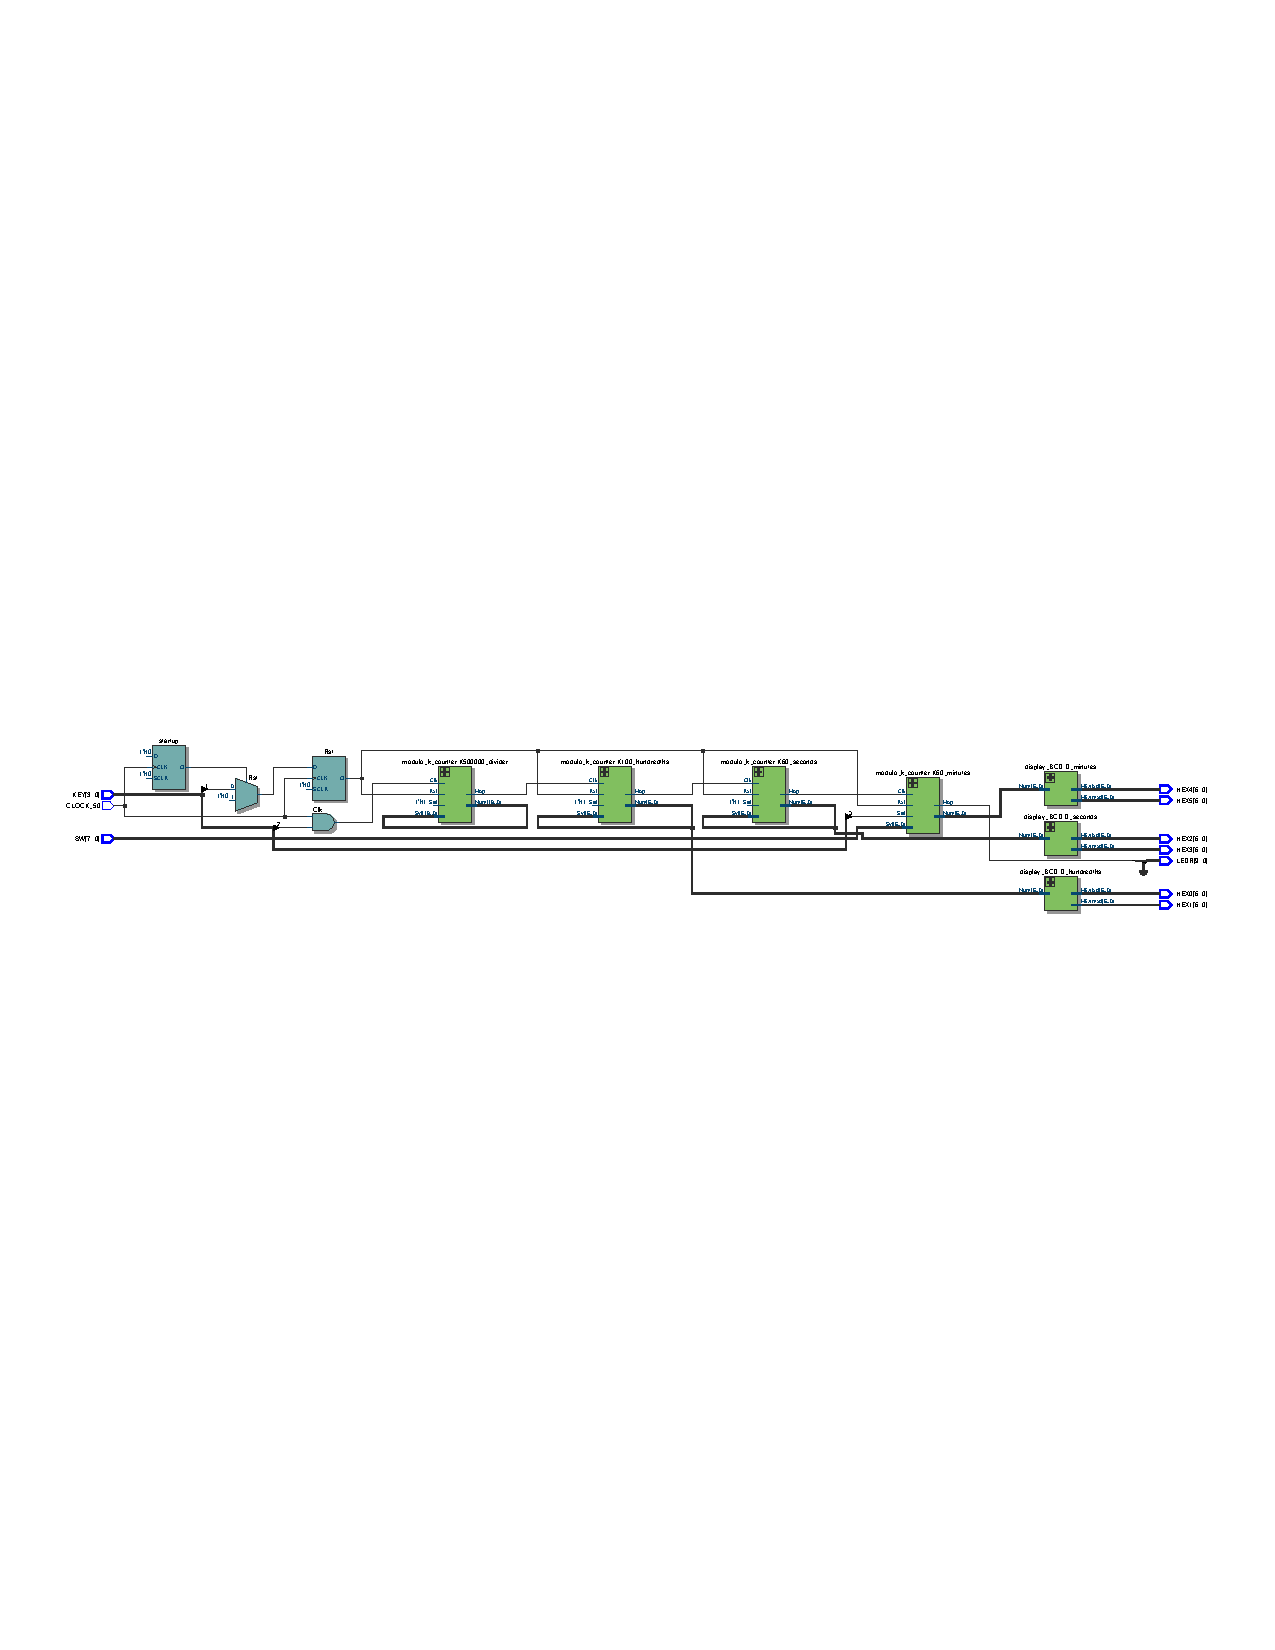
\includegraphics[width=1\textwidth]{Figures/Part2_RTL_TLE.jpg}
    \figcaption{RTL of the TLE}
    \label{fig:p2_RTL_TLE}
\end{figure}

\hfill

\begin{figure}[h]
    \centering
    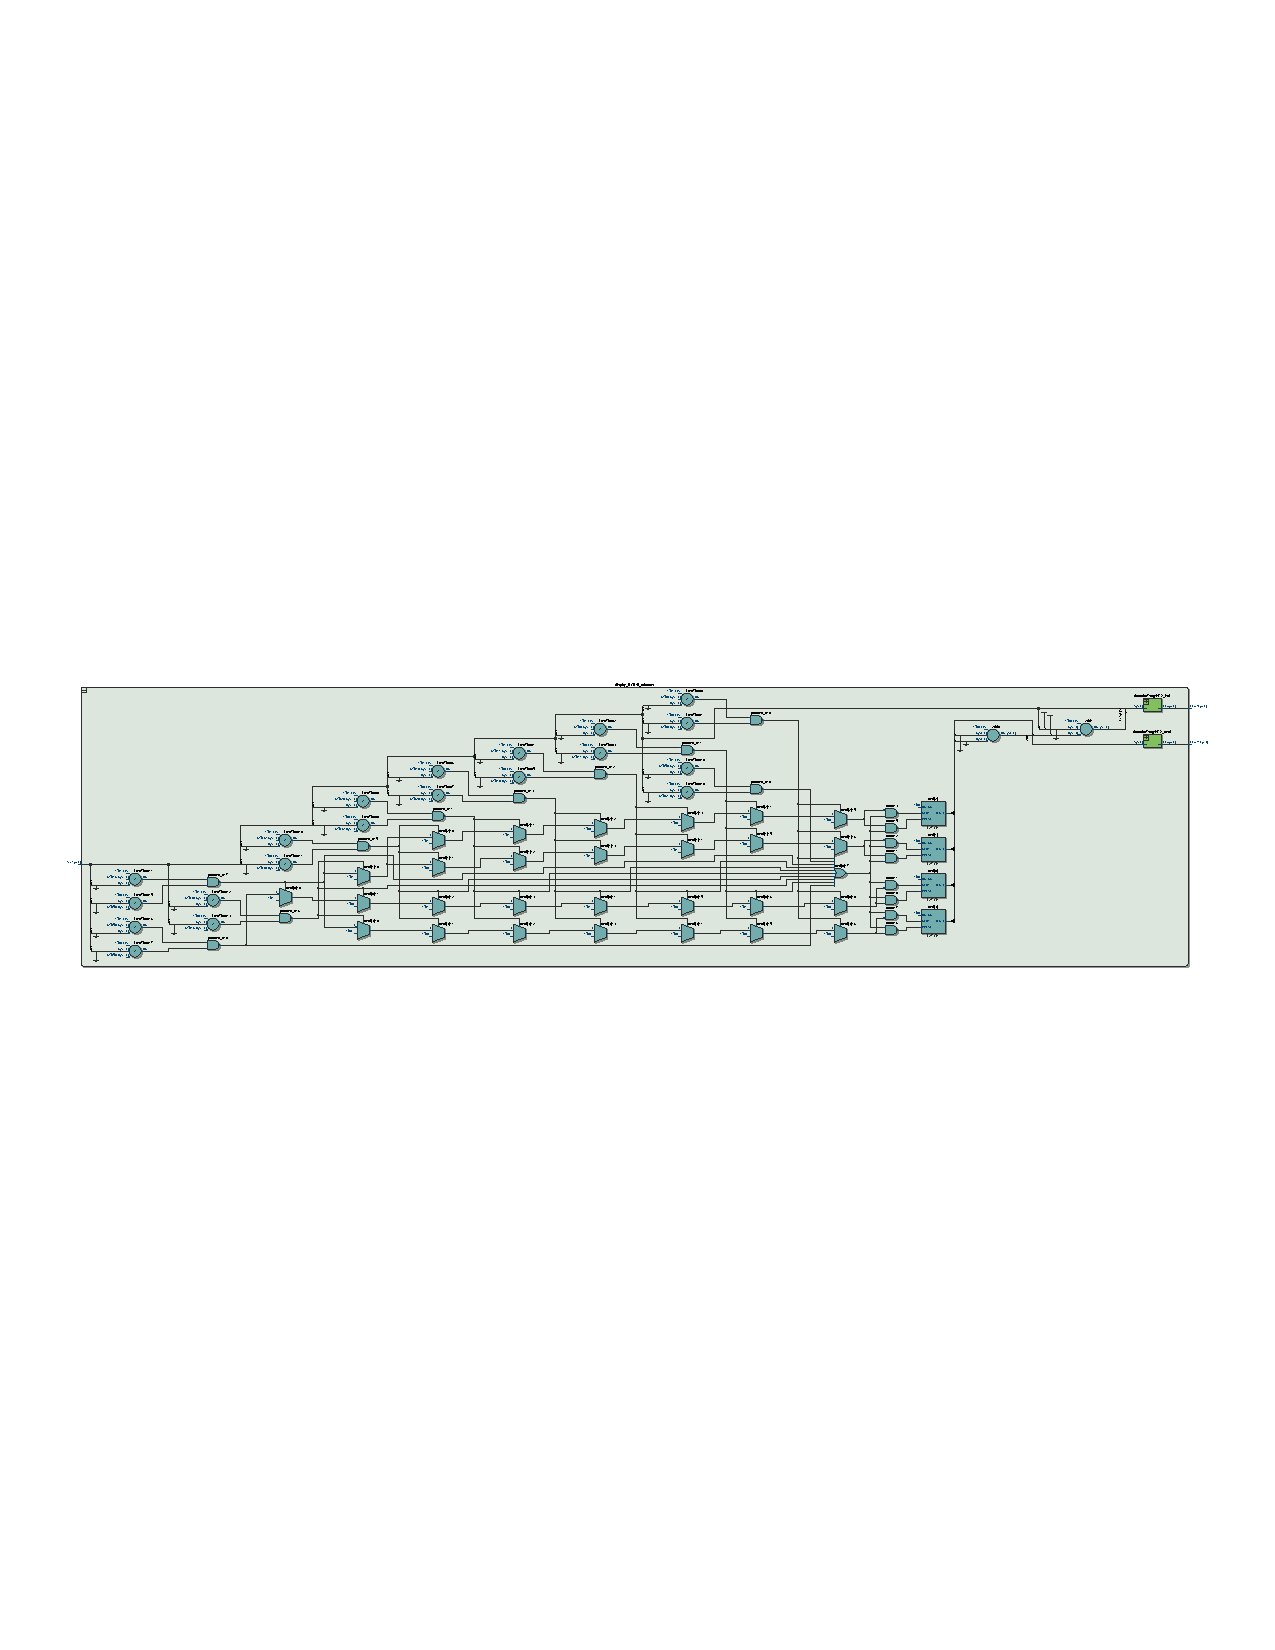
\includegraphics[width=1\textwidth]{Figures/Part2_RTL_BCD_display.jpg}
    \figcaption{RTL of the BCD}
    \label{fig:p2_RTL_BCD}
\end{figure}

RTL of the 7 segment display decoders is not included as this is from previous labs and not important for this lab. As always available on \linkgithub{the GitHub}.

\clearpage
\begin{figure}[h]
    \centering
    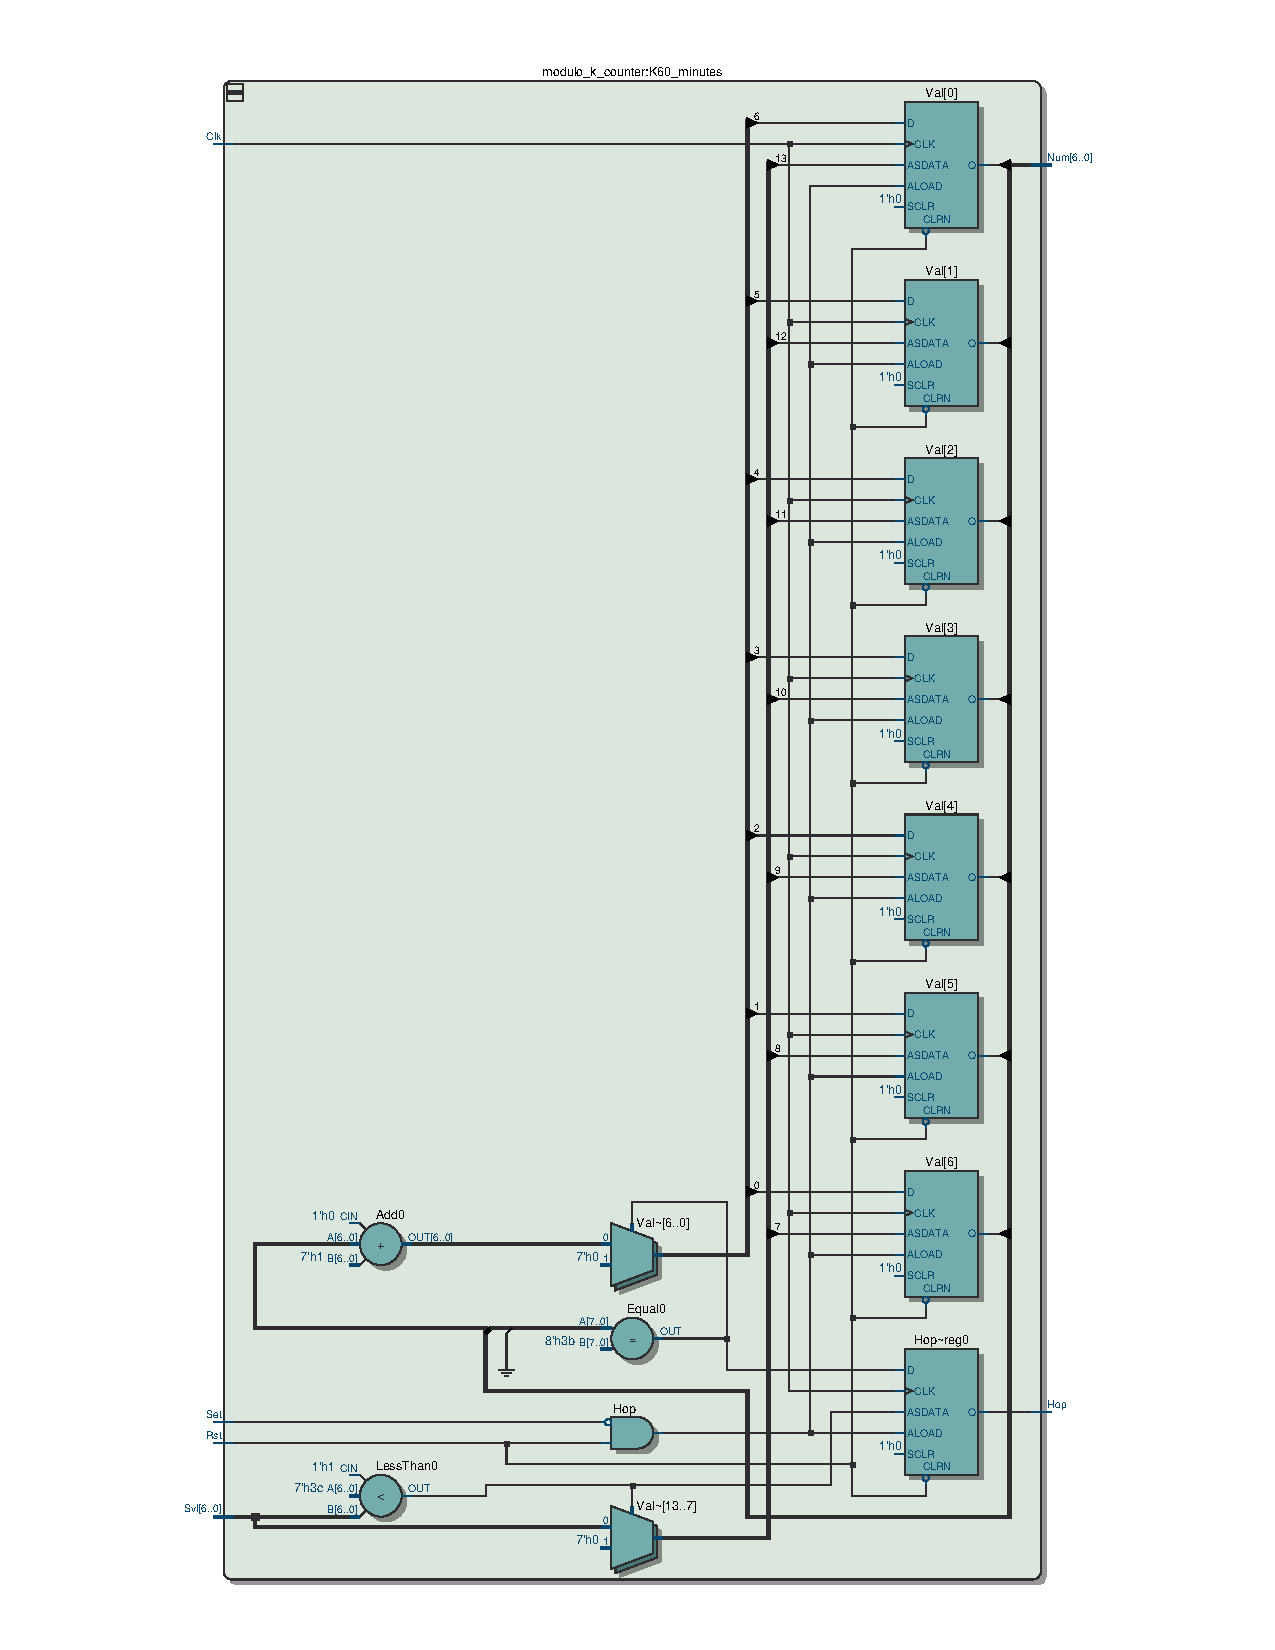
\includegraphics[width=0.8\textwidth]{Figures/Part2_RTL_minute_counter.jpg}
    \figcaption{RTL of the generic counter}
    \label{fig:p2_RTL_Counter}
\end{figure}


\clearpage
\subsection{Results}
It proved to be inefficient to take still pictures of a clock and therefore is a video uploaded instead to YouTube. You can watch it \href{https://youtu.be/4qAZzqxC_Sc?si=TP4QpGwuQ4AIIG2A}{here}. \par
Full url: \url{https://youtu.be/4qAZzqxC_Sc?si=TP4QpGwuQ4AIIG2A}

%   ############################## Section ##############################
\section{Part 3}
The purpose of this task was to make a morse code generator for the first 8 letters of the alphabet, using the provided codes morse and the structure as described by the diagram.


\subsection{Solving}
Solving this was hard with my current knowledge on VHDL, therefore I set on a path to re-learn VHDL to really understand how everything works as it is different to the higher level programming. I had many issues with either trying to sync to different clock events, or trying to drive logic from multiple processes. I also found the hint codes very hard to follow and decided to make everything from scratch myself. The result was using a FSM (Finite State Machine) and making different states based on the current state and other conditions. A sketch of how these states should transfer to each other was made and after compiling, the state exported diagram shown if figure~\ref{fig:state} ended up virtually identical. \par

The logic behind each module is that everything runs on the fast clock and that enable signals is sent during one clock cycle between all modules. There is enable signals for shifting the selected letter by one spot and at the same time decreasing the size. There is also a enable signal to Load new letter in from the selector. The reset is asynchronous but that is probably not visibly measurable as the clock is running at \(\unit[50]{MHz}\). The only thing from the diagram that is not implemented is the \(2\) bit counter as the functionality from implementing it separate instead of just counting and using the main clock seems to serve no additional purpose and was therefore omitted as readability was a higher priority.


\subsection{Code}
\writecode[VHDL]{Part3_TLE.vhd}{TLE Connecting the components and I/O}

\clearpage
\writecode[VHDL]{Part3_logic.vhd}{Logic component controlling the state}

\clearpage
\writecode[VHDL]{Part3_letter_selection.vhd}{Letter selection component}

\clearpage
\writecode[VHDL]{Part3_letter_size.vhd}{Letter size component}

\clearpage
\writecode[VHDL]{Part3_letter_shift.vhd}{Letter shift component}


\clearpage
\subsection{State and RTL}

\begin{figure}[h]
    \centering
    \includegraphics[width=1\textwidth]{Figures/Part3_State.jpg}
    \figcaption{FSM diagram from Quartus}
    \label{fig:state}
\end{figure}

Unfortunately the RTL is very limited in this document as insane resolution is not feasible. There is a possibility to get a rough overview using the following figures, but a fully  no-loss resizeable,  pdf exports, of all the the RTL views is found on \linkgithub{the GitHub} 
inside the following path: \verb|PLK_lab/Lab05/Extra/RTL_exports|.

\hfill

\begin{figure}[h]
    \centering
    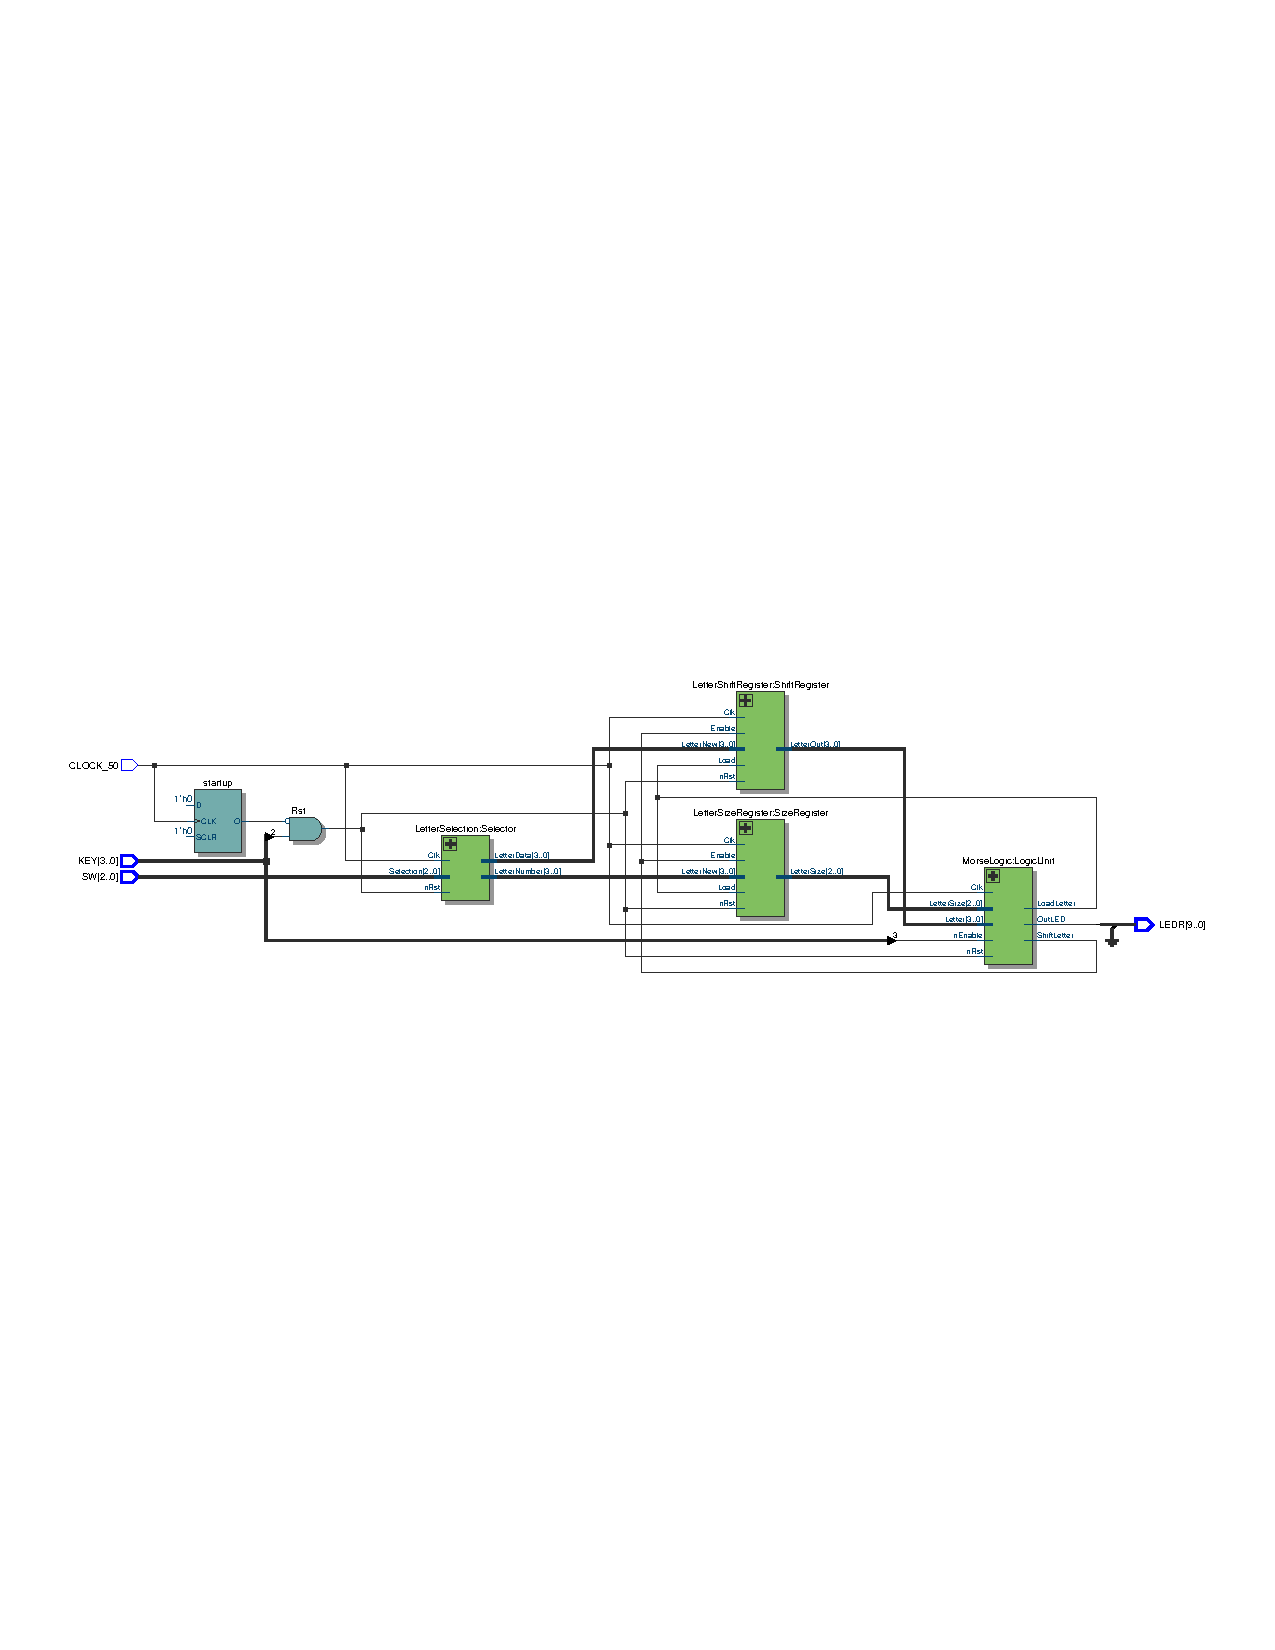
\includegraphics[width=1\textwidth]{Figures/Part3_RTL_TLE.jpg}
    \figcaption{RTL of the TLE}
    \label{fig:p3_RTL_TLE}
\end{figure}

\clearpage
\begin{figure}[h]
    \centering
    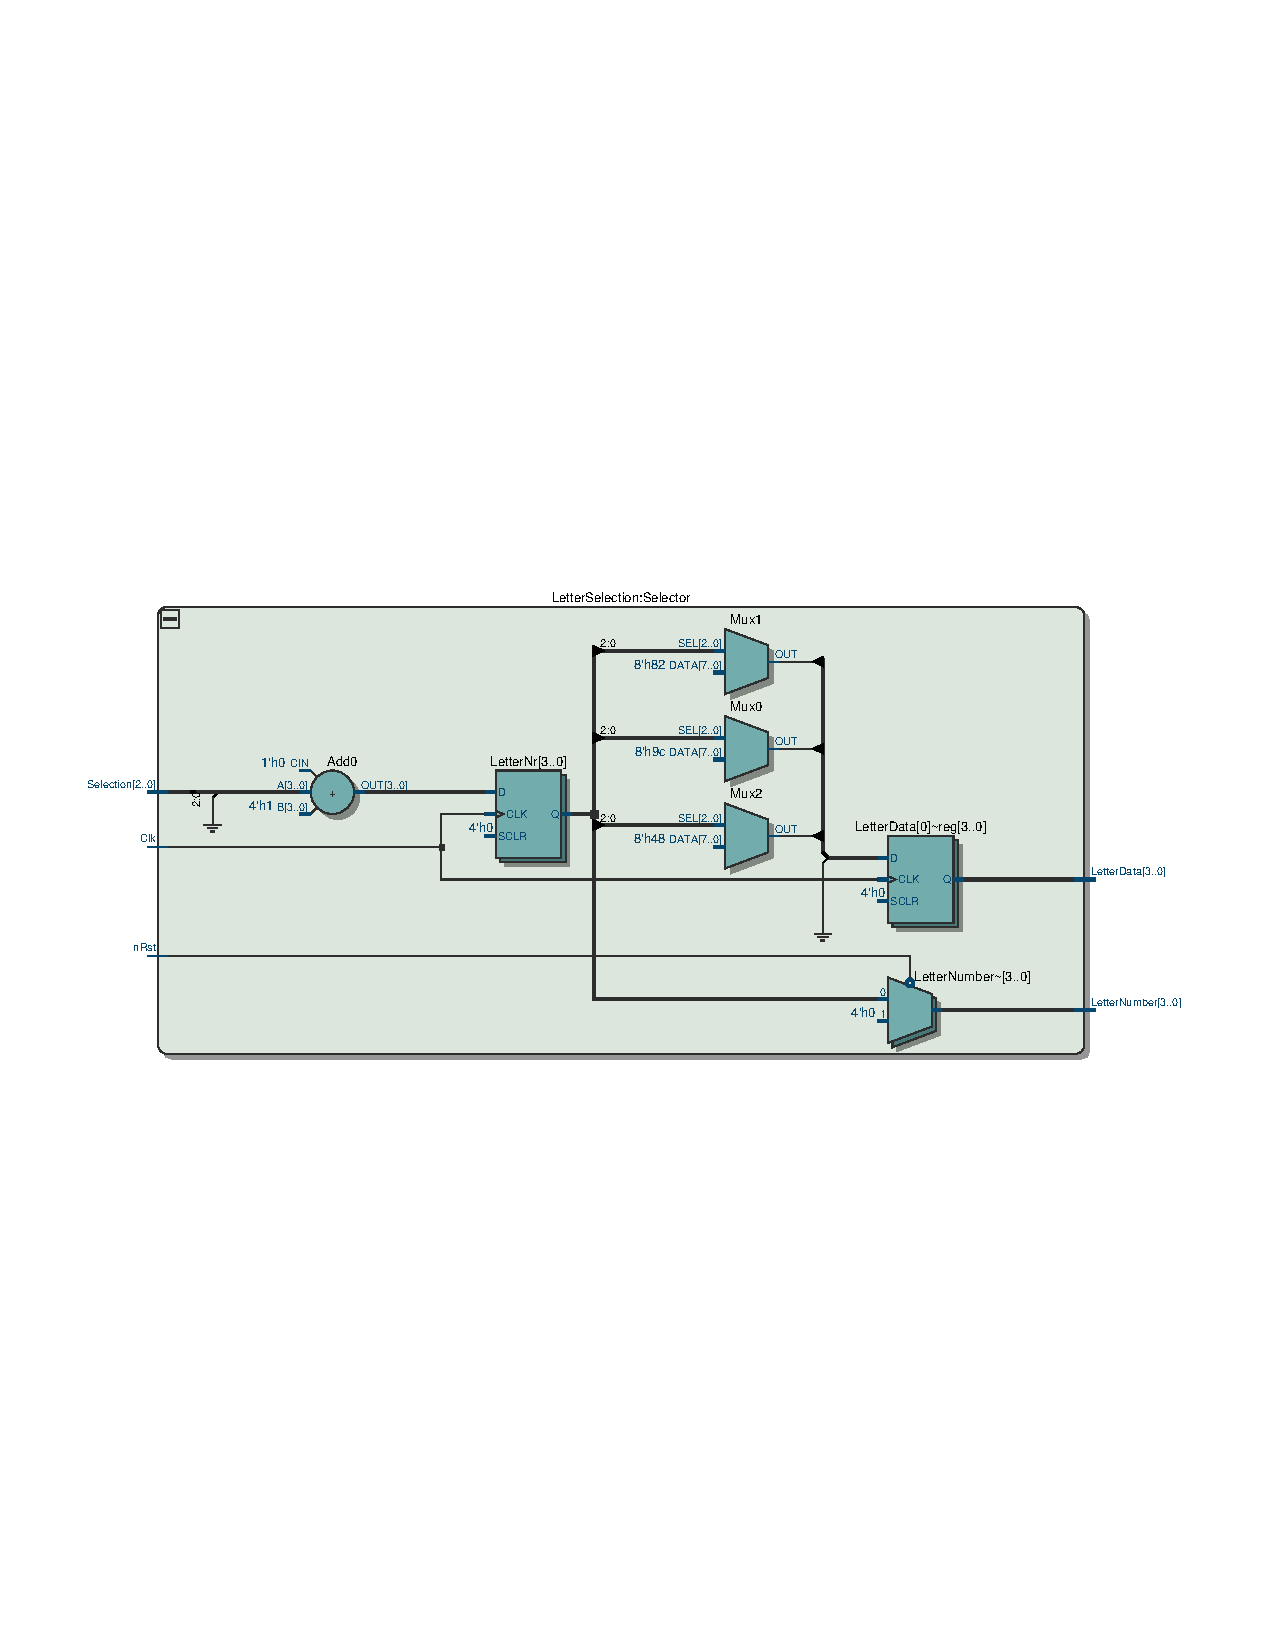
\includegraphics[width=1\textwidth]{Figures/Part3_RTL_Selector.jpg}
    \figcaption{RTL of the letter selector}
    \label{fig:p3_RTL_Sel}
\end{figure}

\hfill

\begin{figure}[h]
    \centering
    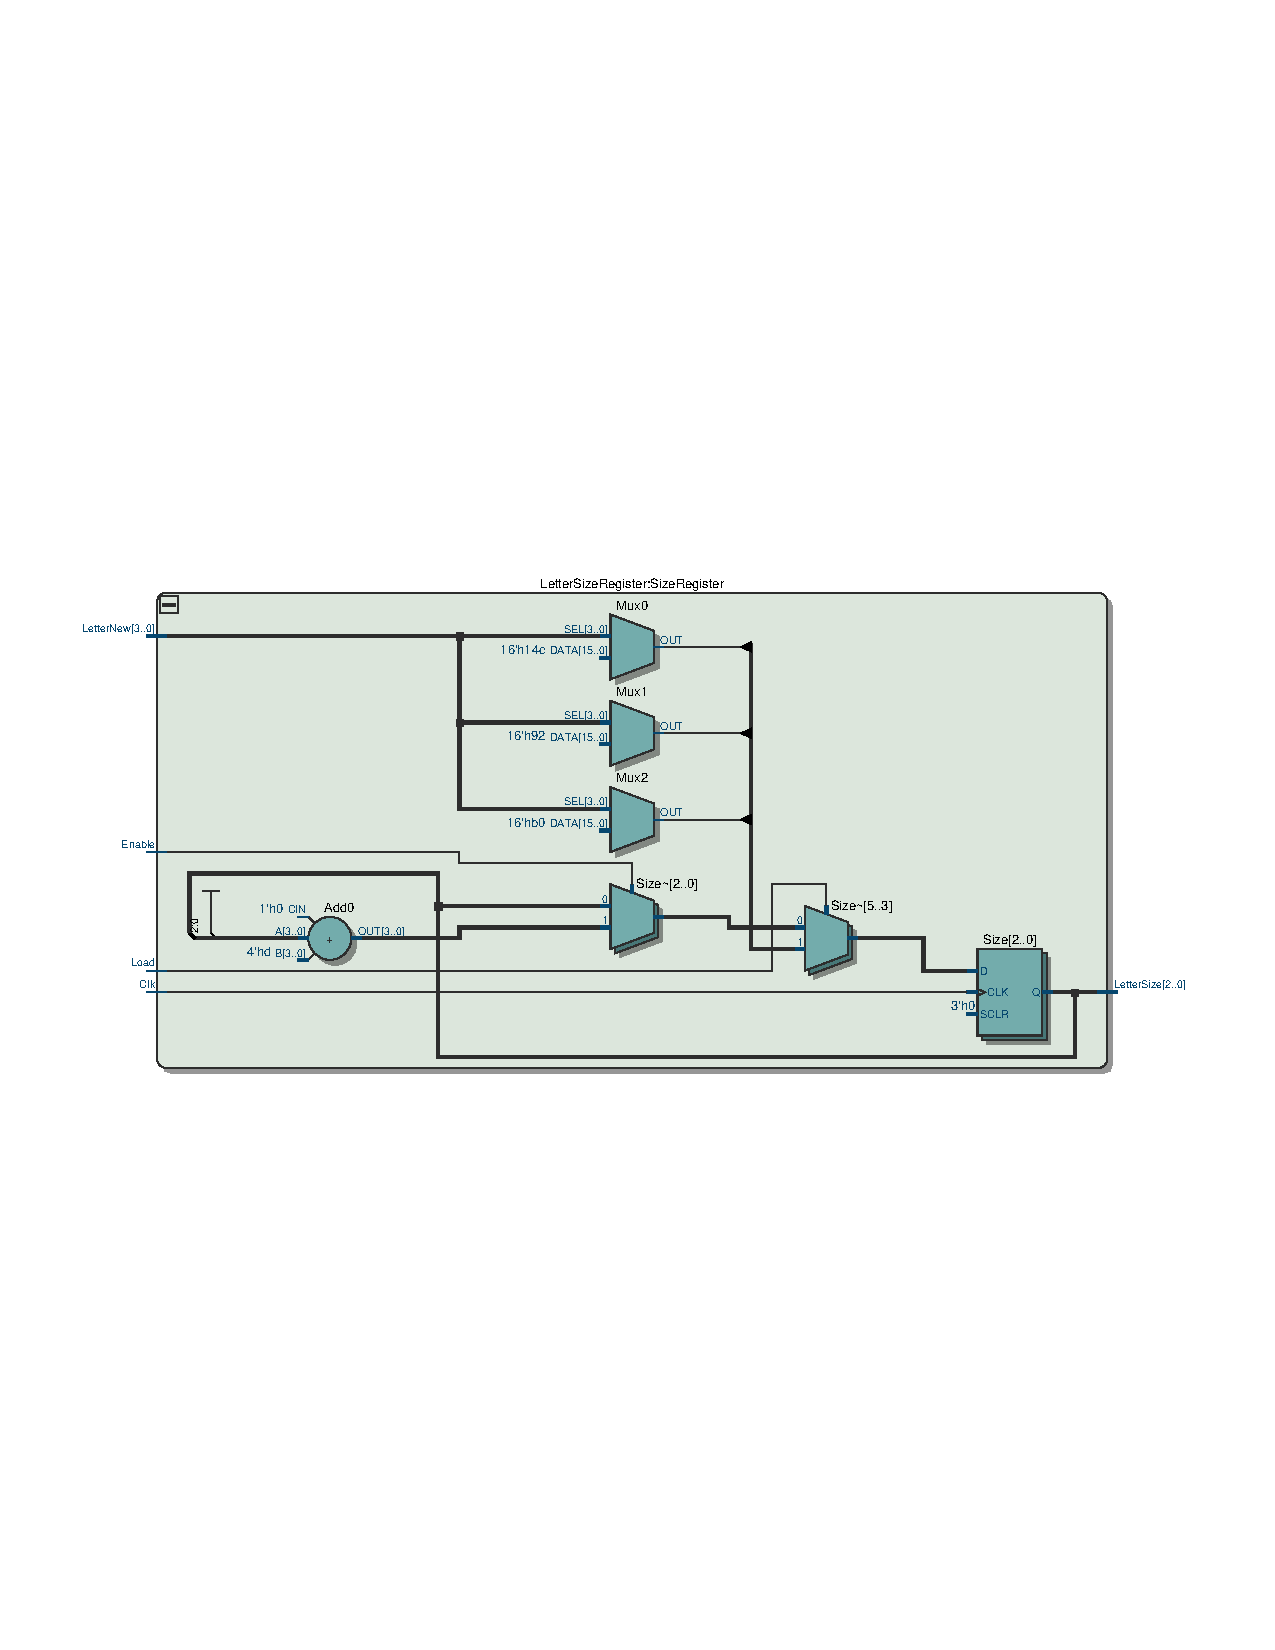
\includegraphics[width=1\textwidth]{Figures/Part3_RTL_Size.jpg}
    \figcaption{RTL of the letter size register}
    \label{fig:p3_RTL_Size}
\end{figure}

\clearpage
\begin{figure}[h]
    \centering
    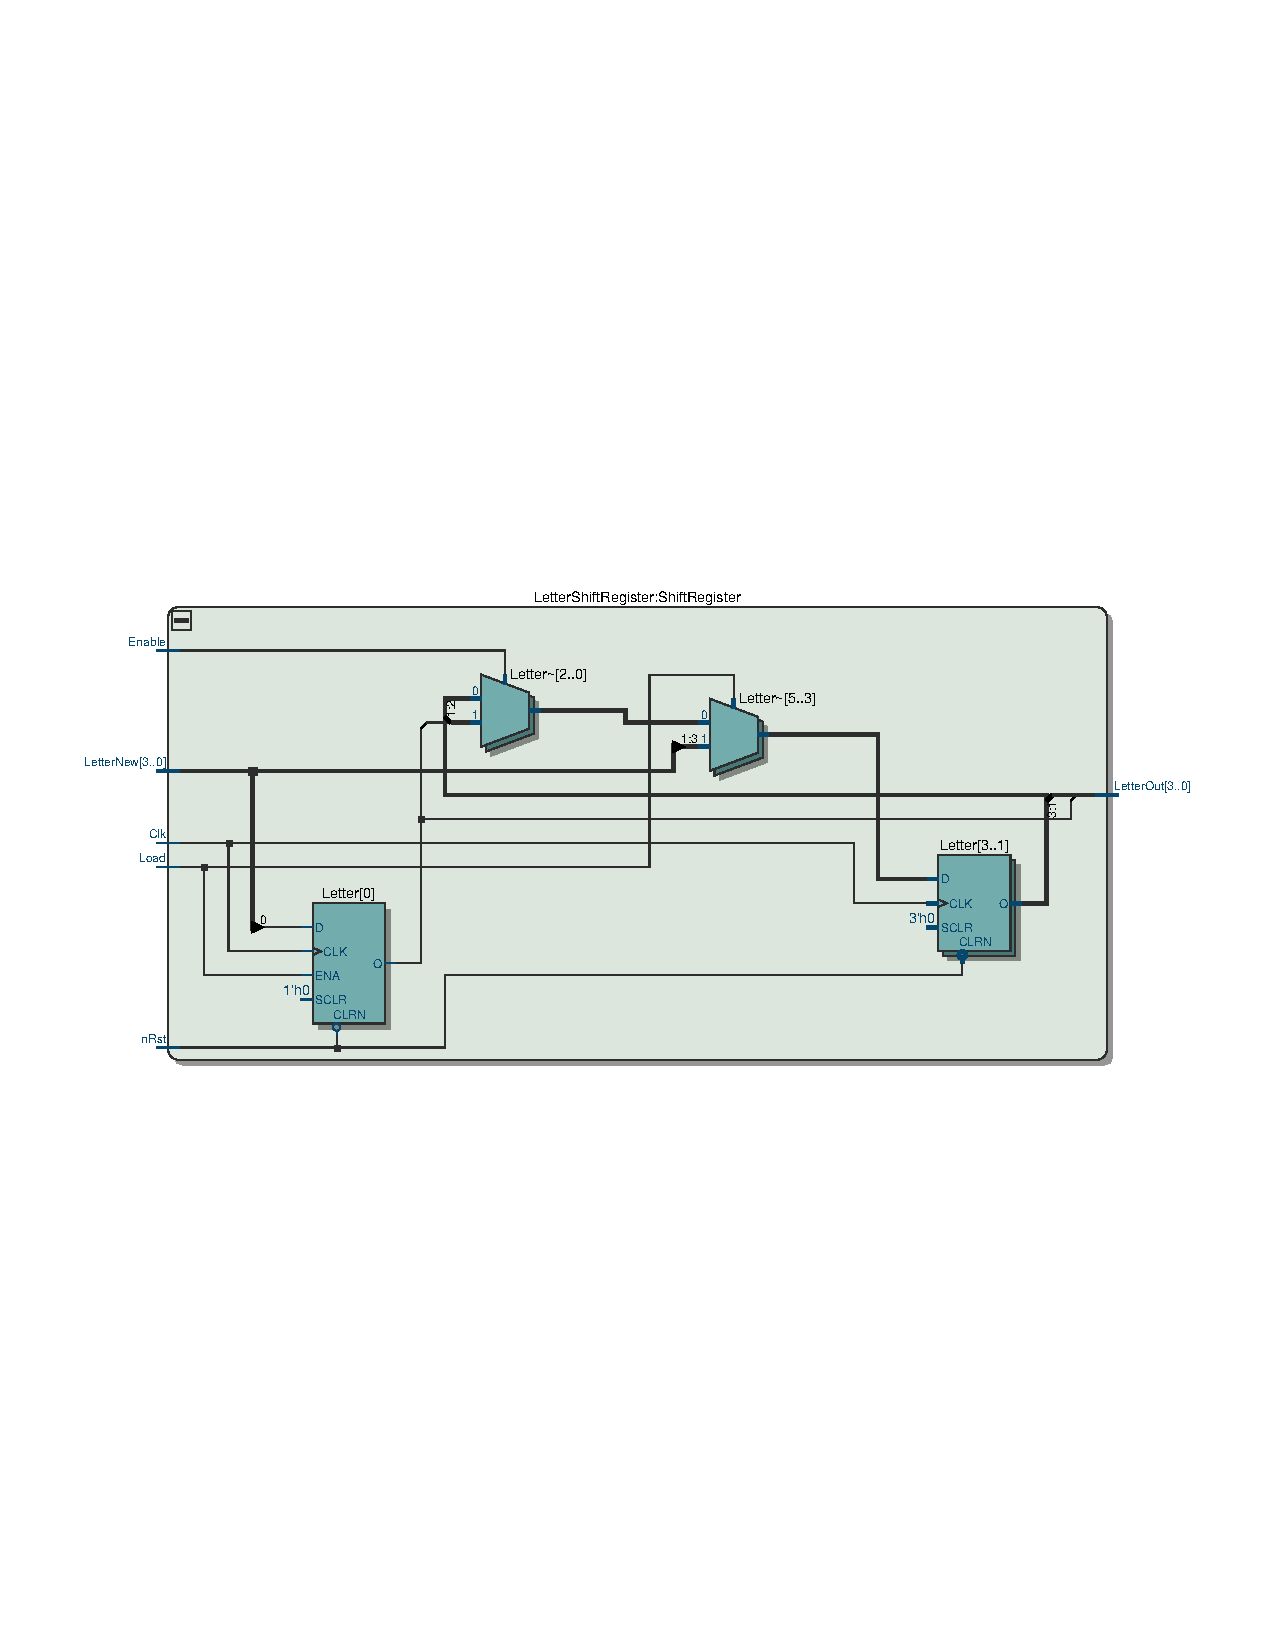
\includegraphics[width=1\textwidth]{Figures/Part3_RTL_Shifter.jpg}
    \figcaption{RTL of the letter shift register}
    \label{fig:p3_RTL_Shift}
\end{figure}

\clearpage
\begin{figure}[h]
    \centering
    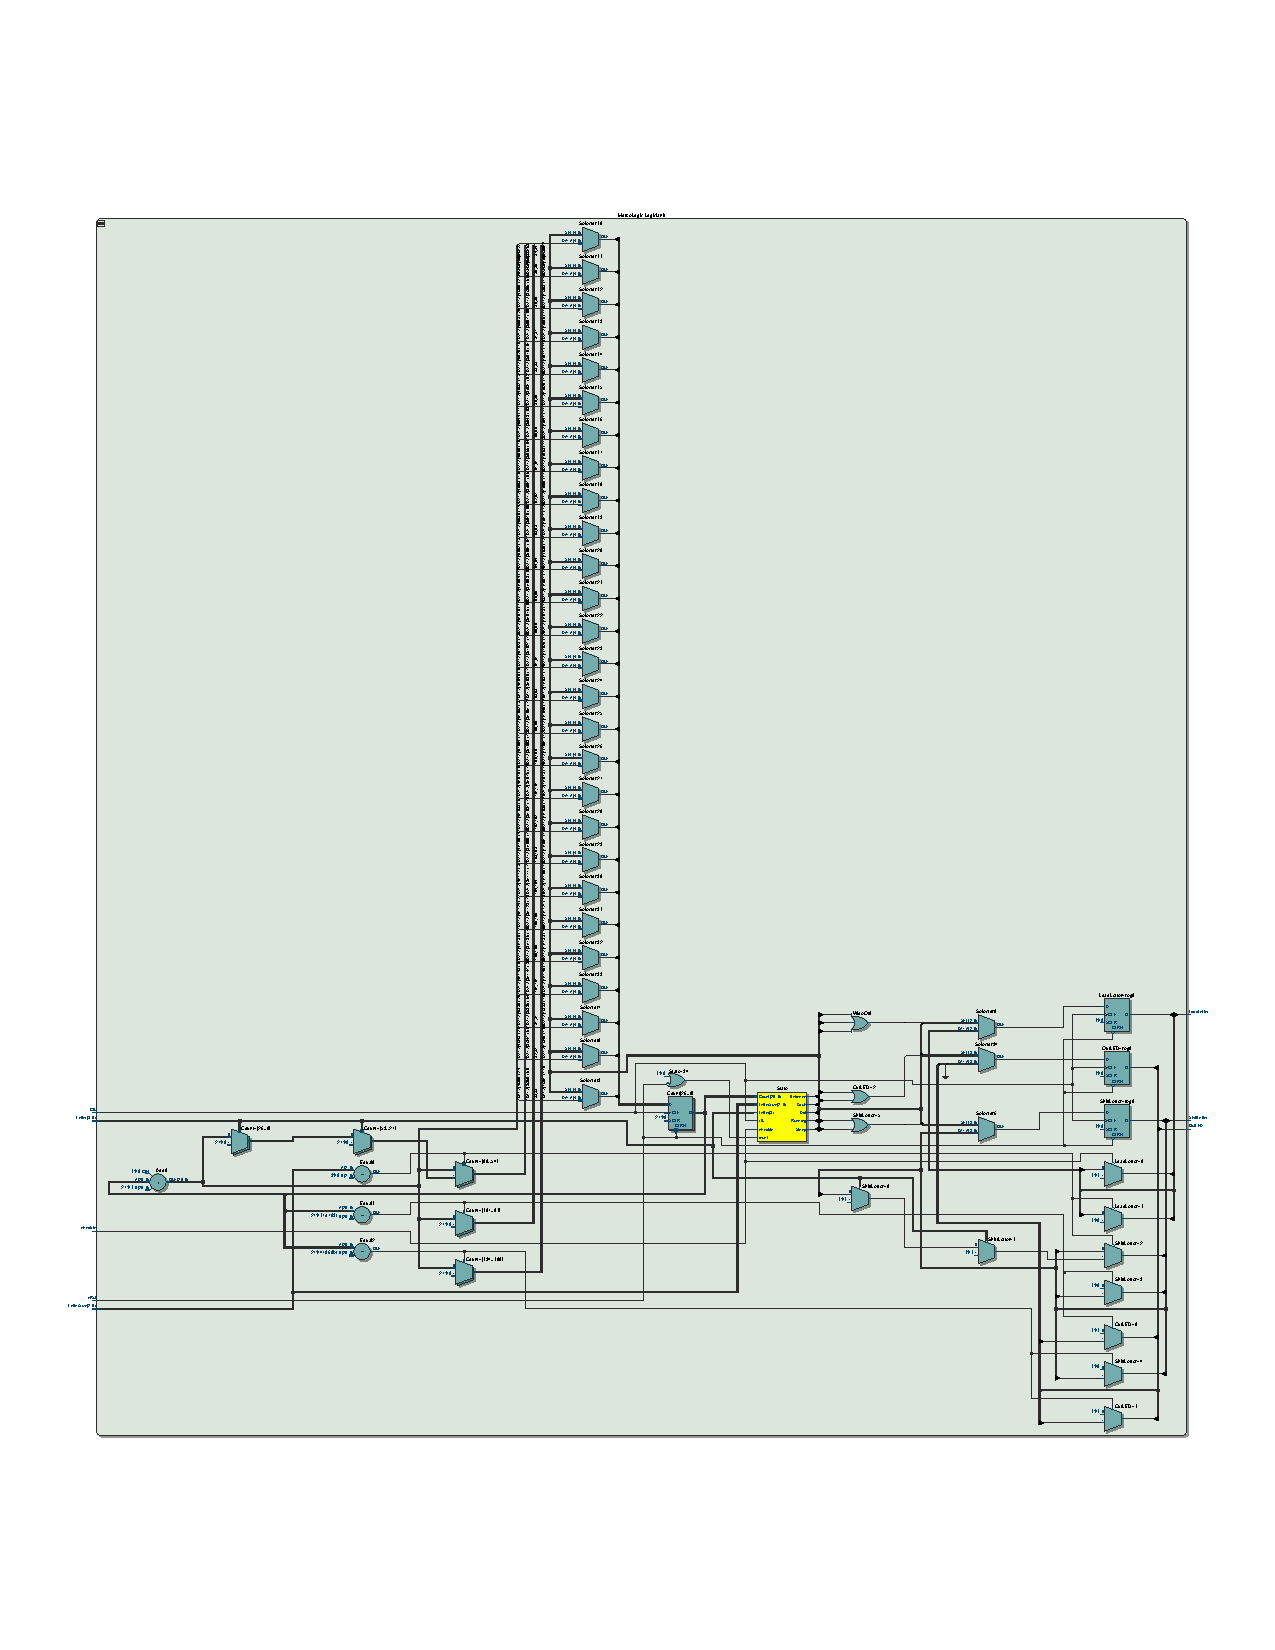
\includegraphics[width=1\textwidth]{Figures/Part3_RTL_Logic.jpg}
    \figcaption{RTL of the Logic}
    \label{fig:p3_RTL_Logic}
\end{figure}

\subsection{Results}
It proved to be inefficient to take still pictures of a timed sequence and therefore is a video uploaded instead to YouTube. You can watch it \href{https://youtu.be/hirlx2AdUFk?si=sx53VB_D5rsin8en}{here}. \par
Full url: \url{https://youtu.be/hirlx2AdUFk?si=sx53VB_D5rsin8en}

\end{document}
